\frame
{
\frametitle{Introduction}


 We want to assess the accuracy (bias, standard error, etc.) of an arbitrary estimate $\hat{\theta}$ knowing only one sample $\mathbf{x}=(x_1,\cdots,x_n)$ drawn from an unknown population  density function $f$.

\begin{itemize}
\item We propose here one way, called \textit{Bootstrap}, to do it using computer intensive techniques for resampling. 

\

\item Bootstrap is a data based simulation method for statistical inference. The basic idea of bootstrap is to use the sample data to compute a statistic and to estimate its sampling distribution, without any model assumption. 

\

\item No theoretical calculations of standard errors needed so we don't care how mathematically  complex the estimator $\hat{\theta}$ can be! 

 \end{itemize}



}

\frame
{
\frametitle{Introduction}


\begin{itemize}
\item The (non-parametric) bootstrap method is an application of the plug-in principle.   By \textit{non-parametric}, we mean that only $\mathbf{x}$ is known (observed) and no prior knowledge on the population density function $f$ is available.

\

\item Originally, the Bootstrap was introduced to compute standard error of an arbitrary estimator by  Efron (1979) and to-date the basic idea remains the same.
\

\item The term \alert{bootstrap} derives from the phrase \textit{to pull oneself up by one's bootstrap} (Adventures of Baron Munchausen, by Rudolph Erich Raspe). The Baron had fallen to the bottom of a deep lake. Just when it
looked like all was lost, he thought to pick himself up by his own
bootstraps.

%\item It is not the same as the term .bootstrap. used in computer science to .boot. a computer from a set of core instructions (though the derivation is similar).
\end{itemize}


}

%%%%%%%%%%%%%%%%%%%%%%%%%%%%%%%%%%%%%%%%%%%%%%%%%%%%%%%%


\frame
{
\frametitle{Bootstrap samples and replications}

\begin{definition}
A \alert{bootstrap sample} $\mathbf{x}^{*}=(x^{*}_{1},x^{*}_{2},\cdots,x^{*}_{n})$ is obtained by randomly sampling $n$ times, with replacement, from the original data points $\mathbf{x}=(x_{1},x_{2},\cdots,x_{n})$.
\end{definition}

\begin{exampleblock}{}
Considering a sample $\mathbf{x}=(x_1,x_2,x_3,x_4,x_5)$, some bootstrap samples can be: 
$$
\begin{array}{l}
\mathbf{x}^{*(1)}=( x_{2},x_{3},x_{5},x_{4},x_{5})\\
\mathbf{x}^{*(2)}=( x_{1},x_{3},x_{1},x_{4},x_{5})\\
\mathrm{etc.}\\
\end{array}
$$
\end{exampleblock}
\begin{definition}
With each bootstrap sample $\mathbf{x}^{*(1)}$ to  $\mathbf{x}^{*(B)}$, we can compute a \alert{bootstrap replication} $\hat{\theta}^{*}(b)=s(\mathbf{x}^{*(b)})$ using the plug-in principle. 
\end{definition}

}
%%%%%%%%%%%%%%%%%%%%%%%%%%%%%%%%%%%%%%%%%%%%%
\frame
{
\frametitle{How to compute Bootstrap samples}

\begin{block}{}
Repeat $B$ times: 
\begin{enumerate}
\item A random number device selects integers $i_1,\cdots, i_n$ each of which equals any value between 1 and $n$ with probability $\frac{1}{n}$.
\item Then compute $\mathbf{x}^{*}=(x_{i_1},\cdots,x_{i_n})$.
\end{enumerate}
\end{block}

\begin{exampleblock}{Some matlab code available on the web}
See BOOTSTRAP MATLAB TOOLBOX, by Abdelhak M. Zoubir and D. Robert Iskander, 
 
\href{http://www.csp.curtin.edu.au/downloads/bootstrap_toolbox.html}{http://www.csp.curtin.edu.au/downloads/bootstrap\_toolbox.html}
\end{exampleblock}


}
%%%%%%%%%%%%%%%%%%%%%%%%%%%%%%%%%%%%%%%%%%%%%%%%%%%%%%
\frame{
\frametitle{How many values are left out of a bootstrap resample ?}
Given a sample $\mathbf{x}=(x_1,x_2,\cdots,x_n)$ and assuming that all $x_i$ are different, the probability that a particular value $x_i$ is left out of a resample $\mathbf{x}^{*}=(x_1^{*},x_2^{*},\cdots,x_n^{*})$ is:
$$
\mathcal{P}(x_{j}^{*}\neq x_i, 1\leq j \leq n)=\left(1-\frac{1}{n}\right)^n
$$
since $\mathcal{P}(x_{j}^{*}=x_i)=\frac{1}{n}$. 
 When $n$ is large, the probability  $\left(1-\frac{1}{n}\right)^n$  converges to $e^{-1}\approx 0.37$. 

%It also means that the expected proportion of values $x_i$s that are not represented in a particular resample $\mathbf{x}^{*}$ is  $\left(1-\frac{1}{n}\right)^n$.

} 
%%%%%%%%%%%%%%%%%%%%%%%%%%%%%%%%%%%%%%%%%%%%%%%%%%%%%%
%\frame{
%\frametitle{Bootstrap replications}
%\begin{definition}
%With each bootstrap sample $\mathbf{x}^{*(1)}$ to  $\mathbf{x}^{*(B)}$, we can compute a \alert{bootstrap replication} $\hat{\theta}^{*}(b)=s(\mathbf{x}^{*(b)})$ using the plug-in principle. 
%\end{definition}

%\begin{exampleblock}{What is the probability that  $\hat{\theta}^{*}(b)=\hat{\theta}$ ?}
%From the previous slide, the probability of that a bootstrap replication is identical to the estimate $\hat{\theta}$ is:
%$$
%\mathcal{P}(\hat{\theta}^{*}(b)=\theta)=1-\left(1-\frac{1}{n}\right)^n
%$$
%When $n$ large, $\mathcal{P}(\hat{\theta}^{*}(b)=\theta)=0.632$
%\end{exampleblock}
%}

%%%%%%%%%%%%%%%%%%%%%%%%%%%%%%%%%%%%%%%%%%%%%%%%%%%%%%
\frame{
\frametitle{The Bootstrap algorithm for Estimating standard errors}

\begin{beamercolorbox}[wd=\linewidth, rounded=true,shadow=true]{postit}
\begin{enumerate}
\item Select $B$ independent bootstrap samples $\mathbf{x}^{*(1)}, \mathbf{x}^{*(2)}, \cdots, \mathbf{x}^{*(B)}$ drawn from $\mathbf{x}$ 
\item Evaluate the bootstrap replications:
$$ 
\hat{\theta}^{*}(b)=s(\mathbf{x}^{*(b)}), \quad \forall b \in \lbrace 1,\cdots,B \rbrace
$$

\item Estimate the standard error $\mathrm{se}_{f}(\hat{\theta})$ by the standard deviation of the $B$ replications:
$$ 
\hat{\mathrm{se}}_{B}=\left\lbrack \frac{\sum_{b=1}^{B}\lbrack \hat{\theta}^{*}(b)-\hat{\theta}^{*}(\cdot)\rbrack^{2}}{B-1} \right\rbrack^{\frac{1}{2}}
$$
where $\hat{\theta}^{*}(\cdot)=\frac{\sum_{b=1}^{B} \hat{\theta}^{*}(b)}{B}$
\end{enumerate}
\end{beamercolorbox}
}
%%%%%%%%%%%%%%%%%%%%%%%%%%%%%%%%%%%%%%%%%%%%%%%%%%%%%
\frame{
\frametitle{Bootstrap  estimate of the standard Error}
\begin{exampleblock}{Example A}
From the distribution  $f$: $f(x)=0.2\ \mathcal{N}(\scriptstyle \mu=1,\sigma=2 \displaystyle) +0.8\  \mathcal{N}( \scriptstyle\mu=6,\sigma=1 \displaystyle)
$. We draw the sample  $\mathbf{x}=(x_1,\cdots,x_{100})$ :
\tiny
$$
\mathbf{x}=
\left\lbrace
\begin{array}{ccccc}
   7.0411 &  4.8397 &  5.3156 &  6.7719 &  7.0616 \\
    5.2546 &   7.3937 &  4.3376 &   4.4010&    5.1724\\
    7.4199 &   5.3677 &  6.7028 &   6.2003 &   7.5707\\
    4.1230 &   3.8914 &   5.2323 &  5.5942 &    7.1479\\
  3.6790 &     0.3509 &   1.4197&   1.7585 &   2.4476\\
   -3.8635 &   2.5731 &   -0.7367 &  0.5627 &   1.6379\\
   -0.1864 &   2.7004 &   2.1487 &  2.3513 &   1.4833\\
   -1.0138 &  4.9794 &  0.1518 &  2.8683 &  1.6269 \\
    6.9523 & 5.3073 &  4.7191 &   5.4374 &   4.6108 \\
    6.5975 &  6.3495 & 7.2762 &  5.9453 &   4.6993\\
    6.1559&  5.8950 &  5.7591 &  5.2173 &   4.9980\\
    4.5010 &  4.7860 &  5.4382 &   4.8893&  7.2940\\
    5.5741 &  5.5139 &  5.8869 &  7.2756 &   5.8449 \\
    6.6439 &  4.5224 &  5.5028 &  4.5672 &  5.8718 \\
    6.0919 &  7.1912 &  6.4181 &  7.2248 &  8.4153 \\
    7.3199 &  5.1305 &  6.8719 &  5.2686 &   5.8055 \\
    5.3602 &  6.4120 &  6.0721 &  5.2740 &  7.2329\\
    7.0912 &  7.0766 &  5.9750 &  6.6091 &  7.2135 \\
    4.9585 &  5.9042 &  5.9273 &  6.5762 &   5.3702\\
    4.7654 &  6.4668 &  6.1983 &  4.3450 &   5.3261\\
\end{array}\right\rbrace
$$
\normalsize
We have $\mu_f=5$ and $\overline{x}=4.9970$.

\end{exampleblock}
}
%%%%%%%%%%%%%%%%%%%%%%%%%%%%%%%%%%%%%%%%%%%%%%%%%%%%%
\frame{
\frametitle{Bootstrap  estimate of the standard Error}

\begin{exampleblock}{Example A}
\begin{enumerate}
\item $B=1000$ bootstrap samples $\lbrace \mathbf{x}^{*(b)}\rbrace $
\item $B=1000$ replications $\lbrace\overline{x}^{*}(b)\rbrace$
\item Bootstrap estimate of the standard error:
$$
\widehat{\mathrm{se}}_{B=1000}=\left\lbrack \frac{\sum_{b=1}^{1000}\lbrack \overline{x}^{*}(b)-\overline{x}^{*}(\cdot)\rbrack^{2}}{1000-1} \right\rbrack^{\frac{1}{2}}=0.2212
$$
where $\overline{x}^{*}(\cdot)=5.0007$.
This is to compare with $\hat{se}(\overline{x})=\frac{\hat{\sigma}}{\sqrt{n}}=0.22$.

\end{enumerate}

\end{exampleblock}
}
%%%%%%%%%%%%%%%%%%%%%%%%%%%%%%%%%%%%%%%%%%%%%%%%%%%%%%%%
\frame
{
\frametitle{Distribution of $\hat{\theta}$}

\begin{block}{}
When enough bootstrap resamples have been generated, not only the standard error but any aspect of the distribution  of the estimator $\hat{\theta}=t(\hat{f})$ could be estimated. One can draw a histogram of the distribution of  $\hat{\theta}$ by using the observed $\hat{\theta}^{*}(b),\ b=1,\cdots,B $. 
\end{block}

\begin{exampleblock}{Example A}

\begin{figure}[!h]
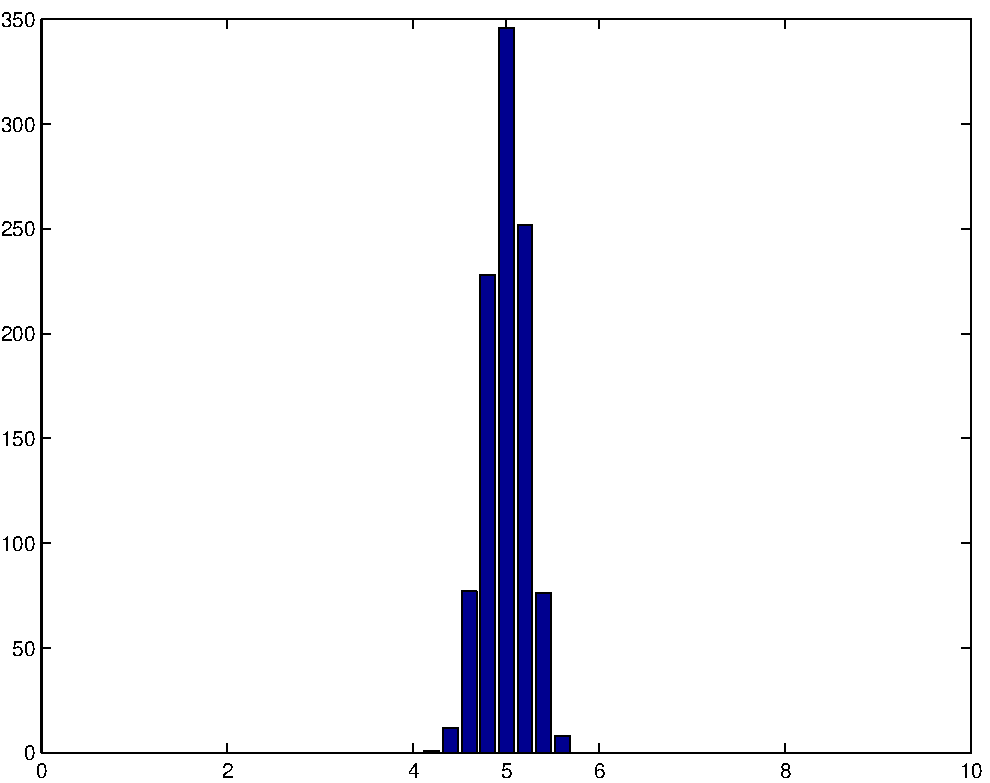
\includegraphics[width=.4\linewidth]{histoExampleA.pdf}
\caption{\small Histogram of the replications $\lbrace\overline{x}^{*}(b)\rbrace_{b=1\cdots B}$. }
\end{figure}
\end{exampleblock}

}
%%%%%%%%%%%%%%%%%%%%%%%%%%%%%%%%%%%%%%%%%%%%%%%%%%%%%%%%%%%%%%
\frame
{
\frametitle{Bootstrap estimate of the standard error}

\begin{definition}
The ideal bootstrap estimate $\mathrm{se}_{\hat{f}} (\hat{\theta}^{*})$ is defined as:
$$
\lim_{B\rightarrow \infty} \hat{\mathrm{se}}_{B}=\mathrm{se}_{\hat{f}} (\hat{\theta}^{*})
$$
 $\mathrm{se}_{\hat{f}} (\hat{\theta}^{*})$ is called a \alert{non-parametric bootstrap estimate of the standard error}.
%When $n$ and $B$ large, the hope is that $\hat{\mathrm{se}}_{B}$ will be close to $\mathrm{se}_{\hat{F}} (\theta^{*})$ which will be close to $\mathrm{se}_{F}(\theta)$.
\end{definition}
}

%%%%%%%%%%%%%%%%%%%%%%%%%%%%%%%%%%%%%%%%%%%%%%%%%%%%%5
\frame{
\frametitle{Bootstrap  estimate of the  standard Error}

\begin{block}{How many $B$ in practice ?}
you may want to limit the computation time.
In practice, you get a good estimation of the standard error for $B$ in between 50 and 200.  
\end{block}
\begin{exampleblock}{Example A}
\begin{table}[!h]
\begin{tabular}{|c|c|c|c|c|c|c|c|}
\hline
$B$& 10& 20 & 50 & 100 & 500 & 1000  & 10000\\
\hline
$\widehat{\mathrm{se}}_{B}$& 0.1386 & 0.2188 & 0.2245 & 0.2142 & 0.2248& 0.2212 & 0.2187\\
\hline
\end{tabular}
\caption{Bootstrap standard error w.r.t. the number $B$ of bootstrap samples.}
\end{table}

\end{exampleblock}
}



%%%%%%%%%%%%%%%%%%%%%%%%%%%%%%%%%%%%%%%%%%%%%%%%%%%%%%%%%%%%%%
\frame{
\frametitle{Bootstrap estimate of bias}
\begin{definition}
The \alert{bootstrap estimate of bias} is defined to be the estimate:
 $$
\begin{array}{ll}
\mathrm{Bias}_{\hat{f}}(\hat{\theta})&=\mathbb{E}_{\hat{f}}\lbrack s(\mathbf{x}^{*})\rbrack-t(\hat{f})\\
&\\
&= \hat{\theta}^{*}(\cdot)-\hat{\theta}
\end{array}
$$
%Here $t(\hat{F})$ may differ from the plug-in estimate $\hat{\theta}$ i.e. $\mathrm{Bias}_{\hat{F}}$ is the plug-in estimate of $\mathrm{Bias}_{F}$ whether or not $\hat{\theta}$ is the plug-in estimate of $\theta$.
\end{definition}

\begin{exampleblock}{Example A}

\small
\begin{table}[!h]
\begin{tabular}{|l|c|c|c|c|c|c|c|}
\hline
B & 10 & 20 & 50 & 100 & 500 & 1000 & 10000 \\
\hline
$\mathbb{E}_{\hat{f}}(\overline{x}^{*})$ & 5.0587 & 4.9551 &5.0244 & 4.9883 &  4.9945 & 5.0035 & 4.9996 \\
\hline
$\widehat{\mathrm{Bias}}$ & 0.0617 & -0.0419 & 0.0274 & -0.0087 & -0.0025 &  0.0064 &0.0025 \\
\hline
\end{tabular}
\caption{$\widehat{\mathrm{Bias}}$ of  $\overline{x}^{*}$ ($\overline{x}=4.997$ and $\mu_f=5$). }
\end{table}
\end{exampleblock}
}
%%%%%%%%%%%%%%%%%%%%%%%%%%%%%%%%%%%%%%%%%%%%%%%%%%%%%%%%%%%%%%
\frame{
\frametitle{Bootstrap estimate of bias}
\begin{beamercolorbox}[wd=\linewidth, rounded=true,shadow=true]{postit}
\begin{enumerate}
\item $B$ independent bootstrap samples $\mathbf{x}^{*(1)}, \mathbf{x}^{*(2)}, \cdots, \mathbf{x}^{*(B)}$ drawn from $\mathbf{x}$ 
\item Evaluate the bootstrap replications:
$$ 
\hat{\theta}^{*}(b)=s(\mathbf{x}^{*(b)}), \quad \forall b \in \lbrace 1,\cdots,B \rbrace
$$
\item Approximate the bootstrap expectation :
$$
\hat{\theta}^{*}(\cdot)=\frac{1}{B} \sum_{b=1}^{B} \hat{\theta}^{*}(b)=\frac{1}{B} \sum_{b=1}^{B} s(\mathbf{x}^{*(b)})
$$
\item the bootstrap estimate of bias based on $B$ replications is:
$$
\widehat{\mathrm{Bias}}_{B}=\hat{\theta}^{*}(\cdot)-\hat{\theta}
$$
\end{enumerate}
\end{beamercolorbox}
}
%%%%%%%%%%%%%%%%%%%%%%%%%%%%%%%%%%%%%%%%%%%%%%%%%%%%%%%%%%%%%
\frame{
\frametitle{Confidence interval}

\begin{definition}
Using the bootstrap estimation of the standard error, the $100(1-2\alpha)$\%
confidence interval is:
$$
\theta=\hat{\theta} \pm z^{(1-\alpha)} \cdot \widehat{\mathrm{se}}_{B}
$$
\end{definition}

\begin{definition}
If the bias in not null,  the \alert{bias corrected 
confidence interval} is defined by:
$$
\theta=(\hat{\theta}-\widehat{\mathrm{Bias}}_{B}) \pm z^{(1-\alpha)} \cdot \widehat{\mathrm{se}}_{B}
$$
\end{definition}
} 

%%%%%%%%%%%%%%%%%%%%%%%%%%%%%%%%%%%%%%%%%%%%%%%%%%%%%%%%%%%%%%
\frame{
\frametitle{Can the bootstrap answer other questions?}
\begin{exampleblock}{The mouse data}


\begin{table}[!h]
\begin{tabular}{|c|c|}
\hline
&\\
 Data (Treatment group) & 94; 197; 16; 38; 99; 141; 23 \\
&\\
\hline
& \\
Data (Control group) & 52; 104; 146; 10; 51; 30; 40; 27; 46 \\
& \\
\hline
\end{tabular}
\caption{The mouse data [Efron]. 16 mice divided assigned to a treatment group (7) or a control group (9). Survival in days following a test surgery. \alert{Did the treatment prolong survival ?} }
\end{table}


\end{exampleblock}
}
%%%%%%%%%%%%%%%%%%%%%%%%%%%%%%%%%%%%%%%%%%%%%%%%%%%%%%%%%%%%%%
\frame{
\frametitle{Can the bootstrap answer other questions?}
\begin{exampleblock}{The mouse data}
%
\begin{table}[!h]
\begin{tabular}{ccccccc}
$B$ &  50   &  100 & 250   & 500 & 1000 & $\infty$ \\
\hline
$\hat{\mathrm{se}}_{B} (\overline{x}_{Treat})$  & 19.72 & 23.63 & 22.32 & 23.79 & 23.02 & 23.36 \\
%median & 32.21 & 36.35 & 34.46 & 36.72 & 36.48 & 37.83 \\
$\hat{\mathrm{se}}_{B} (\overline{x}_{Cont})$  & - & 11.54 & - & - & - & 9.73 \\
 \end{tabular}
\caption{Bootstrap estimates of the standard error for the mean  for the treatment and control groups of the mouse data.}
\end{table} 

\textbf{Standard error of the difference for $B=100$ Bootstrap replications.}
The observed difference is $d^{*}=48$ with an estimated standard error of $\widehat{\mathrm{se}}_{100}(d^*)=38.14$.
The ratio $48/38.14=1.26$ is better (than $d/\mathrm{se}(d)=1.05$ cf.1st lecture) but still insignificant. 




\begin{itemize}

\item Remember in the first lecture, we compute $d=\overline{x}_{Treat}-\overline{x}_{Cont}=30.63$ with a standard error $\hat{se}(d)=28.93$. The ratio was $d/\hat{se}(d)=1.05$ (an insignificant result as measuring $d=0$ is likely possible).

\item Using bootstrap method
\begin{enumerate}
\item  $B$ bootstrap samples $\mathbf{x}_{Treat}^{*(b)}=(x_{Treat\ 1}^{*(b)},\cdots,x_{Treat\ 7}^{*(b)})$ and $\mathbf{x}_{Cont}^{*(b)}=(x_{Cont\ 1}^{*(b)},\cdots,x_{Cont\ 9}^{*(b)})$, $\forall 1\leq b \leq B$

\item $B$ bootstrap replications are computed: $d^{*}(b)=\overline{x}^{*(b)}_{Treat}-\overline{x}^{*(b)}_{Cont}$

\item  The bootstrap  standard error is computed for $B=1400$: $\hat{se}_{B=1400}=26.85$.  
\item The ratio is  $d/\hat{se}_{1400}(d)=1.14$.
\end{enumerate}
\item This is still not a significant result. 
\end{itemize}

\end{exampleblock}
}
%%%%%%%%%%%%%%%%%%%%%%%%%%%%%%%%%%%%%%%%%%%%%%%%%%%%%%%%%%%%%%
%%%%%%%%%%%%%%%%%%%%%%%%%%%%%%%%%%%%%%%%%%%%%%%%%%%%%%%%%%%%%%
\frame
{
\frametitle{The Law school example}

%\small
\begin{table}[!h]
\begin{flushleft}
\begin{tabular}{lcccccccc}
School &   1  &   2 &    3   &  4  &   5  &   6   &  7  &   8  \\
\hline
LSAT (X) & 576  &  635  &  558 &   578  &  666  &  580  &  555   & 661  \\
GPA (Y) &  3.39   &  3.30   &  2.81   &  3.03  &   3.44   &  3.07   &  3.00   &  3.43 \\

&&&&&&&&\\
\end{tabular}

\begin{tabular}{lccccccc}

School &       9   & 10   & 11 &   12  &  13  &  14   & 15 \\
\hline
LSAT (X) &  651   & 605  &  653  &  575   & 545  &  572  &  594 \\
GPA (Y) &    3.36   &  3.13  &   3.12  & 2.74   &  2.76   &  2.88   &  2.96\\

\end{tabular}
\end{flushleft}
\caption{Results of law schools admission practice  for the LSAT and GPA tests. It is believed that these scores are highly correlated. \alert{Compute the correlation and its standard error.}}
\end{table}


}



\frame
{
\frametitle{Correlation}
The correlation is defined :
$$ 
\mathrm{corr}(X,Y)=\frac{\mathbb{E}\lbrack (X -\mathbb{E}(X)) \cdot (Y -\mathbb{E}(Y))\rbrack }{\left( \mathbb{E} \lbrack (X -\mathbb{E}(X))^2 \rbrack  \cdot \mathbb{E} \lbrack (Y -\mathbb{E}(Y))^2 \rbrack \right)^{1/2}}
$$ 

Its typical estimator is:
$$
\widehat{\mathrm{corr}}(\mathbf{x},\mathbf{y})=\frac{\sum_{i=1}^{n} x_i\ y_i - n\ \overline{x}\ \overline{y}}{\lbrack \sum_{i=1}^{n}x_i^2-n\overline{x}^2 \rbrack^{1/2}\cdot \lbrack\sum_{i=1}^{n} y_i^2-n \overline{y}^2 \rbrack^{1/2} }
$$

}


\frame{
\frametitle{The Law school example}
\begin{itemize}
\item The estimated correlation is $\widehat{\mathrm{corr}}(\mathbf{x},\mathbf{y})=.7764$ between LSAT and GPA. 
%\item Precise theoretical formula for the standard error of the estimator is unavailable.
\end{itemize}
\begin{exampleblock}{Non-parametric Bootstrap estimate of the standard error}

\begin{table}[!h]
\begin{tabular}{l|cccccccc}
$B$ & 25 & 50 & 100 & 200 & 400 & 800 & 1600 & 3200 \\
\hline
$\hat{\mathrm{se}}_B$& .140 & .142 & .151 & .143 & .141 &.137 & .133 & .132 \\
\end{tabular}
\caption{Bootstrap estimate of standard error for $\widehat{\mathrm{corr}}(\mathbf{x},\mathbf{y})=.776$.}
\end{table}
The standard error stabilizes to $\mathrm{se}_{\hat{f}} (\widehat{\mathrm{corr}})\approx.132$.  
\end{exampleblock}
}

%%%%%%%%%%%%%%%%%%%%%%%%%%%%%%%%%%%%%%%%%%%%%%%%%%%%%%%
\frame{
\frametitle{The Law school example: Conclusion}

\begin{itemize}
\item The textbook formula for  the correlation coefficient is:
 $$
\hat{\mathrm{se}}(\widehat{\mathrm{corr}})=(1-\widehat{\mathrm{corr}}^2)/\sqrt{n-3}
$$
\item With $\widehat{\mathrm{corr}}=0.7764$, the standard error is $\hat{se}(\widehat{\mathrm{corr}})=0.1147$.
\item The estimated non-parametric bootstrap  standard error $\mathrm{se}_{B=3200}$ is $0.132$.
%\item The parametric bootstrap  standard error for $B=3200$ is $0.1169$.
\end{itemize}

}
%%%%%%%%%%%%%%%%%%%%%%%%%%%%%%%%%%%%%%%%%%%%%%%%%%%%%%%%
%%%%%%%%%%%%%%%%%%%%%%%%%%%%%%%%%%%%%%%%%%%%%%%%%
\frame{
\frametitle{Non-Parametric Bootstrap}

\begin{figure}[!h]
$$
\begin{array}{rcr}
Real\ World & & Bootstrap\ World \\
&&\\
f \rightarrow \mathbf{x}  & \Rightarrow & \hat{f} \rightarrow \mathbf{x}^{*} \\
&&\\
\downarrow & & \downarrow \ \\
&&\\
\hat{\theta} & & \hat{\theta}^{*}\\
\end{array} 
$$
\caption{Unknown probability model $f$ gives observed data $\mathbf{x}$ and we wish to know the accuracy of the statistic $\hat{\theta}=s(\mathbf{x})$ for estimating the parameter of interest $\theta=t(f)$. No prior information is available on $f$, therefore $\hat{f}$ is estimated from $\mathbf{x}$ as the empirical distribution function. Accuracy is inferred from observed variability of bootstrap replication $\hat{\theta}^{*}=s(\mathbf{x}^{*})$.}
\end{figure}

}

%%%%%%%%%%%%%%%%%%%%%%%%%%%%%%%%%%%%%%%%%%%%%%%%%%%%%%%%%
\frame
{
\frametitle{Parametric Bootstrap}

\begin{figure}[!h]
$$
\begin{array}{rcccr}
Real\ World & & Estimation & & Bootstrap\ World \\
&&&&\\
Prior: f\simeq \mathcal{N}(\mu,\sigma) \rightarrow \mathbf{x}  & \Rightarrow & (\overline{x},\hat{\sigma})& & \hat{f}\simeq\mathcal{N}(\overline{x},\hat{\sigma}) \rightarrow \mathbf{x}^{*} \\
&&&&\\
\downarrow &&& & \downarrow \ \\
&&&&\\
\hat{\theta} && & & \hat{\theta}^{*}\\
\end{array} 
$$
\caption{Example of parametric Bootstrap. $f$ is a normal distribution of unknown parameters $(\mu, \sigma)$. From the observed data $\mathbf{x}$ drawn from $f$, an estimation of the parameters  is performed giving $(\overline{x},\hat{\sigma})$.
$\hat{f}$ is then modelled by a normal distribution $\mathcal{N}(\overline{x},\hat{\sigma})$, from which bootstrap replications can be drawn $\mathbf{x}^{*}$.  Accuracy is inferred from observed variability of bootstrap replication $\hat{\theta}^{*}=s(\mathbf{x}^{*})$.}
\end{figure}
}




%%%%%%%%%%%%%%%%%%%%%%%%%%%%%%%%%%%%%%%%%%%%%%%%%%%%%%%%%%%%%%
\frame
{
\frametitle{Summary}
\begin{itemize}
\item Re-sampling of $\mathbf{x}$ to compute bootstrap samples $\mathbf{x}^{*}$ \item Computation of bootstrap replication of the estimator $\hat{\theta}^{*}(b)$ for $b=1,\cdots,B$
\item From replications,  standard error $\widehat{\mathrm{se}}_{B}$, the bias $\widehat{\mathrm{Bias}}_{B}$ and the  confidence interval. 
\item Non-parametric bootstrap estimations (no prior on $f$).
\end{itemize}
}
%%%%%%%%%%%%%%%%%%%%%%%%%%%%%%%%%%%%%%%%%%%%%%%%%%%%%%%%%%%%%%
